\documentclass[10pt]{article}
\usepackage[margin=0.8in]{geometry}
\usepackage{amsmath,amssymb,booktabs,graphicx,hyperref,xcolor}
\hypersetup{colorlinks=true,linkcolor=blue!50!black,urlcolor=blue!50!black}
\setlength{\parskip}{0.4em}\setlength{\parindent}{0pt}
\graphicspath{{../}}
\author{}\date{}
\begin{document}
\title{Phase diagram of the bilayer square-lattice t1--t2--J model from a neural quantum state}\maketitle

Research report, problem2 (\texttt{prompt.tex}). Working directory: \texttt{benchmarks/lattice-gap-mechanism/problem2}. All energies in units of t1 = 1; t2 = 0.2 throughout. Computations started 2026-10-26.

\section*{0. Summary of results}

\begin{itemize}
\item \textbf{Method.} Variational Monte Carlo with a neural quantum state (translation-symmetric RBM $\times$ two-body Jastrow $\times$
geminal/pairing determinant, with a Pfaffian-type triplet block for spin sectors), sampled in fixed
(N$_1$, N$_2$, S\^{}z) sectors, optimized by stochastic reconfiguration; 4$\times$4 bilayer (64 spin-orbitals) for the full
diagram, 6$\times$6 for a finite-size check at half filling; validated against exact diagonalization (2$\times$2: energies to
0.2--0.5 \%, gaps to 0.5--3 \%) and against exact free-fermion energies on 4$\times$4. Every number carries a Monte Carlo
standard error; finite-size gaps are always compared with the exact J = 0 value of the same cluster.
\item \textbf{Half-filling cut ($\nu$ = 1/2).} Three regimes on the 4$\times$4 bilayer: a \textbf{Fermi liquid} for J $\lesssim$ 2.7 (free-band
n(k), gaps at the level spacing); a \textbf{superconductor of interlayer singlet pairs} for 2.7 $\lesssim$ J $\lesssim$ 4.5 (two
distinct variational minima with the paired one lower; single-particle gap open, two-particle gap \emph{below} the
free value, pair-binding energy --1.7 to --3.5, distance-independent pair correlation $\approx$ 0.09--0.15, Fermi
surface washed out); and a \textbf{symmetric gapped insulator} for J $\gtrsim$ 4.5 (two-particle gap 1.7, 2.5, 4.1 at
J = 5, 6, 8, far above the free value 1.17; spin gap 3.2, 4.0, 5.9; single-particle gap 8.5--10.6; pair
correlation back at the free level; n(k) flat; rung singlet weight 83--94 \%; no magnetic or density Bragg peak;
S$_+$($\pi$,$\pi$) $\to$ 0). \textbf{A gapped phase is present on the half-filling cut.} The SC $\to$ insulator boundary agrees with
the second-order strong-coupling estimate (rung-pair gap closes at J $\approx$ 4.9); the FL $\to$ SC boundary with the
BCS estimate of where the interlayer pairing gap exceeds the level spacing.
\item \textbf{Quarter-filling cut ($\nu$ = 1/4).} Fermi liquid up to J = 5 (free n(k), gaps at the 3.63 level spacing, but a
growing pair-binding energy of two \emph{added} electrons), then a \textbf{superconductor of rung pairs} at J = 6--8
(two-particle gap 0.38 $\to$ 0.23 against a free value 3.63, single-particle gap 4.5--5.9, pair correlation 0.12--0.17,
N($\pi$,$\pi$) $\le$ 1.5 so no pair crystal, spin gap 3.9--5.3). No gapped symmetric phase away from half filling.
\item \textbf{($\nu$, J) plane.} The symmetric gapped insulator is confined to the $\nu$ = 1/2 line; it is a Mott insulator of
charge-2e rung pairs at one pair per site, and doping it in either direction gives a rung-pair superfluid. The
superconducting region surrounds it and widens with J; the Fermi liquid holds the weak-coupling corner at every
filling (strictly, a superconductor with an exponentially small gap). $\nu$ = 1 is a band insulator. No magnetic or
charge order anywhere (t$_2$ removes the nesting). Phases are symmetric under $\nu$ $\to$ 1--$\nu$; the numbers are not
(t$_2$ $\to$ --t$_2$).
\item \textbf{Spectra at J = 8, $\nu$ = 1/2} (strong-coupling quasiparticle theory, amplitudes exact from two-rung
diagonalization, checked on an exact 3$\times$2 cluster and against the VMC gaps): STM dI/dV shows two quasiparticle
bands (trion/holon, width $\approx$ 3) separated by a single-particle gap $\approx$ 8, with the rung-pair edge at $\approx$ 3.5 inside
it; the local spin spectrum is a triplon band starting at $\Delta$\_s $\approx$ 5.4 (minimum at ($\pi$,$\pi$)) of width $\approx$ 3.3, with the
layer-symmetric channel empty; the resistivity is activated, $\rho$ $\propto$ exp(E\_a/T) with E\_a $\approx$ 3.7 $\approx$ $\Delta$$_2$ (pair channel)
rather than $\Delta$$_1$/2 = 4.0.
\item \textbf{Limits.} 4$\times$4 finite-size gaps of order 1; variational bias $\approx$ 0.02--0.06 per site (40--55 \% of the
second-order correlation energy recovered at weak coupling); the 6$\times$6 check at $\nu$ = 1/2, J = 4 converged for
the ground state (pair correlation halved relative to 4$\times$4, rung-singlet weight up to 75 \%, no Bragg peaks) but
its N $\pm$ 2 sector energies did not converge well enough to give the 6$\times$6 pair gap (Sec. 3.6), so the
superconductor--insulator boundary is best quoted as J\_c2 $\approx$ 4--5.
\end{itemize}

\section*{1. Model and conventions}

H = --t1 $\sum$\_$\langle$ij$\rangle$$\ell$$\sigma$ (c$^\dagger$\_\{i$\ell$$\sigma$\} c\_\{j$\ell$$\sigma$\} + h.c.) -- t2 $\sum$\_$\langle$$\langle$ij$\rangle$$\rangle$$\ell$$\sigma$ (\ldots{}) + J $\sum$\_i S\_\{i1\}$\cdot$S\_\{i2\}, two layers $\ell$ = 1,2, no interlayer hopping. Conserved: N\_1, N\_2 (electrons per layer), S\^{}z, S$^2$. Filling $\nu$ = N/(4 N\_c), N\_c = L$^2$ sites per layer. $\nu$ = 1/2 is one electron per layer per site (N = 2N\_c), $\nu$ = 1/4 is N = N\_c.


\section*{2. Method}


\subsection*{2.1 Variational state (neural quantum state)}

The wavefunction is a real-valued "neural-Jastrow $\times$ geminal" state in the occupation-number basis of the 4N\_c spin-orbitals (site, layer, spin):

$\psi$(n) = det[ $\Phi$(x\_a, y\_b) | U(x\_a) ] $\cdot$ exp( 1/2 n$^T$ W n ) $\cdot$ exp( $\sum$\_\{r$\in$translations\} $\sum$\_\{f=1\}\^{}\{F\} ln cosh(b\_f + $\sum$\_m W\_\{f,m\} n\_\{T\_r m\}) ).

\begin{itemize}
\item $\Phi$(x, y) is a pairing (geminal) function between an occupied up-spin orbital x = (site, layer) and an occupied
down-spin orbital y. It is translation invariant, $\Phi$ = F[$\ell$, $\ell$', $\Delta$r] with the twisted-boundary sign structure,
4 N\_c parameters. It contains the Fermi liquid ($\Phi$ = projector on the filled band, layer diagonal), the interlayer
BCS state $\Phi$\_k = v\_k/u\_k (layer off-diagonal), and the rung-singlet product ($\Phi$ = $\delta$\_\{rr'\}(1--$\delta$\_\{$\ell$$\ell$'\})) as
special points, so the three candidate phases are all in the variational family and the optimizer chooses.
\item U are unpaired orbitals for sectors with N\_$\uparrow$ $\ne$ N\_$\downarrow$ or odd N. For the S\^{}z = 1 sector (spin gap) an additional
antisymmetric up-up pairing block T(x, x') = antisym[cos(q$\cdot$r) G[$\ell$,$\ell$',$\Delta$r]] is included; the resulting Pfaffian is
evaluated exactly through the identity Pf = $\pm$det(M) (r$_1$$^T$ T r$_2$), M = [$\Phi$ | Q], r$_1$,$_2$ the last two rows of M$^-$¹
(verified numerically against a direct Pfaffian). This block is what represents a propagating rung triplon.
\item W is a translation-invariant two-body (density--density, all four flavours) Jastrow factor, 16 N\_c parameters.
\item The last factor is a translation-symmetric restricted Boltzmann machine with F = 16 hidden features per
translation (hidden density $\alpha$ = F/4 = 4), 16$\cdot$4N\_c + 16 parameters.
\end{itemize}
Total $\approx$ 1.4$\cdot$10$^3$ parameters on 4$\times$4 ($\approx$ 3$\cdot$10$^3$ on 6$\times$6).

\subsection*{2.2 Sampler}

Metropolis--Hastings in the fixed sector (N\_1, N\_2, N\_$\uparrow$, N\_$\downarrow$) with two move types: (i) same-layer, same-spin hop between any two sites of a layer (proposal corrected for the number of allowed hops, as in NetKet's exchange rule), probability 0.7; (ii) interlayer spin exchange ($\uparrow$ in layer 1 at site i $\leftrightarrow$ $\downarrow$ in layer 2 at site j), the move generated by the S$^+$\_\{i1\}S$^-$\_\{i2\} term, probability 0.3. The move set conserves all four numbers and is ergodic in the sector. 64 chains, one sample per sweep of 4N\_c proposals, 16 discarded sweeps per chain after each update. Acceptance 0.4--0.6.

\subsection*{2.3 Optimizer}

Stochastic reconfiguration (natural gradient, NetKet \texttt{VMC\_SR}, real mode, explicit quantum geometric tensor) with diagonal shift 0.01, SPRING momentum 0.8, learning rate linearly 0.03 $\to$ 0.01, 2048 samples per step. Every ground state is optimized from two initial states, the free-band Fermi-liquid geminal and the rung-singlet geminal, for 300 steps (200 on the ($\nu$, J) grid); the lower energy is kept and the energy difference between the two optimized states is reported as a metastability indicator. Gap sectors (N $\pm$ 1, N $\pm$ 2, S\^{}z = 1) start either from an interlayer BCS geminal with $\Delta$$_0$ = J/2 (half-filling cut, 300 steps) or from the converged ground-state parameters of the same point (all other points, 150--200 steps; 120 on the grid); the S\^{}z = 1 sector is run with two starts of the triplet block (Fermi-liquid-triplet-dominated and triplon-dominated) and the lower energy is kept. The optimization runs in chunks of 25 steps with parameter checkpoints; a non-finite energy (rare, from a singular step) restores the last checkpoint, halves the learning rate and redraws the Markov chains. Runs whose final estimate has an integrated autocorrelation time above 5, R-hat above 1.05, or a standard error per site above 0.003 + 0.0006 J are discarded and repeated with a new seed (6 of $\approx$ 300 runs). The 6$\times$6 runs use 1024 samples, 120 (ground state) and 80 (gap sector) steps.

\subsection*{2.4 Lattices, boundary conditions, sectors}

L$\times$L bilayers with L = 4 (32 sites, 64 spin-orbitals, 32 electrons at $\nu$=1/2) and L = 6 (72 sites, 144 spin-orbitals, 72 electrons at $\nu$=1/2). Mixed periodic/antiperiodic boundary conditions are chosen per filling so that the non-interacting ground state is a closed shell: for L=4, (P,A) at $\nu$ = 1/8, 3/8, 1/2, 5/8, 7/8 and (A,A) at $\nu$ = 1/4, 3/4; for L=6, (P,A) at $\nu$=1/2 and (P,P) at $\nu$ = 1/4, 3/4. Per point the sectors optimized are: ground state (N\_1 = N\_2 = N/2, S\^{}z = 0); S\^{}z = 1 (spin gap $\Delta$\_s = E(S\^{}z=1) -- E\_0, triplon momentum q = (0,0) and ($\pi$,$\pi$) both tried); N$\pm$2 with one electron added to each layer (two-particle charge gap $\Delta$\_c2 = [E(N+2) + E(N--2) -- 2E(N)]/2); N$\pm$1 (single-particle gap $\Delta$\_c1 = E(N+1) + E(N--1) -- 2E(N)); from these the pair-binding energy E\_pb = E(N+2) + E(N) -- 2E(N+1). On a finite lattice all gaps have a non-interacting (J=0) value set by the level spacing; these exact reference values are shown alongside and the diagnostic is the excess over them.

\subsection*{2.5 Validation against exact diagonalization}

A bit-string exact diagonalization code (\texttt{code/ed.py}) was written for the same term list and checked against NetKet's operator on the 2$\times$2 open bilayer (full spectrum agrees to 10$^-$¹$^3$). On that cluster the VMC state reproduces the exact ground-state energies to 0.2--0.3 \% in every S\^{}z = 0 sector, the S\^{}z=1 sector to 0.25--0.5 \% once the triplon block is included (8.8 \% without it), the spin gap to 0.5 \% and the two-particle charge gap to 3 \% (table \texttt{data/validation\_2x2.md}). On the 4$\times$4 lattice with (P,A) boundaries the J = 0 energy equals the exact filled-band value --3.41421 per site within one standard error (--3.41417(8)), and the S\^{}z = 1 sector with the triplet block reproduces the exact free particle-hole triplet energy (--3.3395(2) versus --3.3410 per site after 15 steps); at J = 0.5 the VMC spin gap 1.170(5) and single-particle gap 1.190(11) match the level spacing 1.172.

\subsection*{2.6 Statistical uncertainties}

Every number from the VMC carries the Monte Carlo standard error of the mean from the final evaluation with 8192 (ground state) or 16384 (gap sectors) samples, computed with NetKet's binning estimate including the integrated autocorrelation time; R-hat < 1.01 in all reported 4$\times$4 runs. Gaps and structure factors are propagated in quadrature. The variational bias (energy above the true ground state) is not included in the error bars; it is estimated from the 2$\times$2 benchmark as $\approx$ 0.2--0.5 \% of the energy and from the two-initialization split.

\section*{3. Half-filling cut ($\nu$ = 1/2)}

Lattice 4$\times$4 bilayer, boundary (P,A), N = 32 electrons (16 per layer), closed shell at J = 0 with a level gap of 1.172 between the highest occupied and lowest empty one-particle level; this value is the finite-size reference for every gap below. Reference energies: free band --3.41421 per site; exact second-order perturbation theory in J on the same cluster (\texttt{code/pt2\_fl.py}) gives E$_2$ = --0.0024, --0.0095, --0.0378 per site at J = 0.5, 1, 2.

\subsection*{3.1 Results along the cut (J = 0.5 \ldots{} 8)}

Energies and gaps, 4x4 bilayer, bc=pa, nu=0.5. Free-band (J=0) references: spin gap 1.172, 2-particle gap 1.172, 1-particle gap 1.172.

\begin{center}\footnotesize\setlength{\tabcolsep}{3pt}
\resizebox{\textwidth}{!}{%
\begin{tabular}{llllllll}\toprule
J & E/site & init (split) & $\Delta$\_s & $\Delta$\_c2 & $\Delta$\_c1 & E\_pb(+) & E\_pb(--) \\ \midrule
0.5 & -3.41551(33) & fl (0.0004) & 1.1702(54) & 1.1584(56) & 1.190(11) & -0.0059(59) & -0.0568(61) \\
1 & -3.41902(46) & sg (0.0014) & 1.211(15) & 1.0675(88) & 1.216(15) & -0.164(13) & -0.133(11) \\
2 & -3.43746(82) & sg (0.0030) & 1.074(18) & 0.833(15) & 1.275(33) & -0.577(40) & -0.308(27) \\
2.5 & -3.4567(12) & sg (0.0023) & 1.085(27) & 0.612(23) & --- & --- & --- \\
3 & -3.4936(19) & sg (0.0262) & 1.114(64) & 0.298(34) & 1.702(68) & -1.726(59) & -1.081(52) \\
3.5 & -3.6008(20) & fl (0.0061) & 1.743(38) & 0.306(37) & --- & --- & --- \\
4 & -3.7821(28) & sg (0.1627) & 2.269(58) & 0.522(49) & 4.056(95) & -3.488(72) & -3.579(76) \\
5 & -4.3294(23) & fl (0.0027) & 3.159(54) & 1.679(43) & --- & --- & --- \\
6 & -4.9667(31) & fl (0.0091) & 4.017(64) & 2.468(54) & 8.45(11) & -6.457(91) & -5.500(89) \\
8 & -6.3298(43) & sg (0.0024) & 5.932(74) & 4.134(72) & 10.61(16) & -6.02(15) & -6.93(13) \\
\bottomrule\end{tabular}}\end{center}

Correlation diagnostics (per site):

\begin{center}\footnotesize\setlength{\tabcolsep}{3pt}
\resizebox{\textwidth}{!}{%
\begin{tabular}{lllllllllll}\toprule
J & $\langle$S\_i1$\cdot$S\_i2$\rangle$ & double occ. & n(k) jump & n(k) in/out & S$_-$($\pi$,$\pi$) & S$_+$($\pi$,$\pi$) & N($\pi$,$\pi$) & P\_pair(r$\ge$2) & P\_pair(L/2,L/2) & P\_pair(0) \\ \midrule
0.5 & -0.00493(85) & 0.24983(77) & 0.999524(96) & 1.00/0.00 & 1.5372(59) & 1.4592(59) & 1.97 & 0.01081(34) & 0.00149(64) & 0.25445(94) \\
1 & -0.00978(77) & 0.24883(90) & 0.99490(30) & 1.00/0.00 & 1.5486(61) & 1.4358(61) & 1.47 & 0.01327(22) & 0.00416(63) & 0.26016(89) \\
2 & -0.02968(88) & 0.24566(86) & 0.97035(76) & 0.98/0.01 & 1.6768(70) & 1.3754(70) & 1.95 & 0.02656(35) & 0.01758(93) & 0.2809(10) \\
2.5 & -0.04725(93) & 0.24056(88) & 0.9326(10) & 0.96/0.03 & 1.7878(65) & 1.3421(65) & --- & 0.03831(36) & 0.02826(93) & 0.3000(11) \\
3 & -0.1261(15) & 0.22008(88) & 0.7143(22) & 0.82/0.10 & 1.9525(80) & 1.1395(80) & 1.69 & 0.09609(45) & 0.0893(13) & 0.3853(16) \\
3.5 & -0.2942(31) & 0.1681(13) & 0.3509(36) & 0.61/0.26 & 2.413(12) & 0.763(12) & --- & 0.15027(66) & 0.1432(18) & 0.5591(30) \\
4 & -0.4879(45) & 0.0956(19) & 0.1738(47) & 0.54/0.37 & 2.981(18) & 0.447(18) & 0.72 & 0.0892(11) & 0.0797(26) & 0.7443(44) \\
5 & -0.6202(28) & 0.0446(13) & 0.0950(49) & 0.52/0.42 & 3.255(19) & 0.233(19) & --- & 0.0271(12) & 0.0169(13) & 0.8713(28) \\
6 & -0.6659(30) & 0.0296(13) & 0.081(11) & 0.51/0.43 & 3.177(20) & 0.153(20) & 0.22 & 0.0114(11) & 0.00533(44) & 0.9160(30) \\
8 & -0.7031(24) & 0.0172(11) & 0.0445(64) & 0.51/0.46 & 3.122(19) & 0.084(19) & 0.14 & 0.0133(19) & 0.0062(13) & 0.9533(24) \\
\bottomrule\end{tabular}}\end{center}

Column key: E/site is the lower of the two optimized states, "init (split)" says which start won and the energy difference per site between the two optimized states; $\Delta$\_s = E(S\^{}z=1) -- E\_0 (minimum over the (0,0), ($\pi$,$\pi$) and triplon-type starts); $\Delta$\_c2 = [E(N+2)+E(N--2)--2E(N)]/2; $\Delta$\_c1 = E(N+1)+E(N--1)--2E(N); E\_pb($\pm$) = E(N$\pm$2)+E(N)--2E(N$\pm$1) (negative: the two added/removed particles bind). All errors are one standard error from the Monte Carlo estimates, propagated; the exact J = 0 value of every gap on this cluster is 1.172. Figures: \texttt{figures/cut\_L4\_nu0.500.png} (all quantities versus J), \texttt{figures/nk\_L4\_nu0.500.png} (momentum distribution), \texttt{figures/Sq\_L4\_nu0.500.png} (spin structure factors).
\begin{center}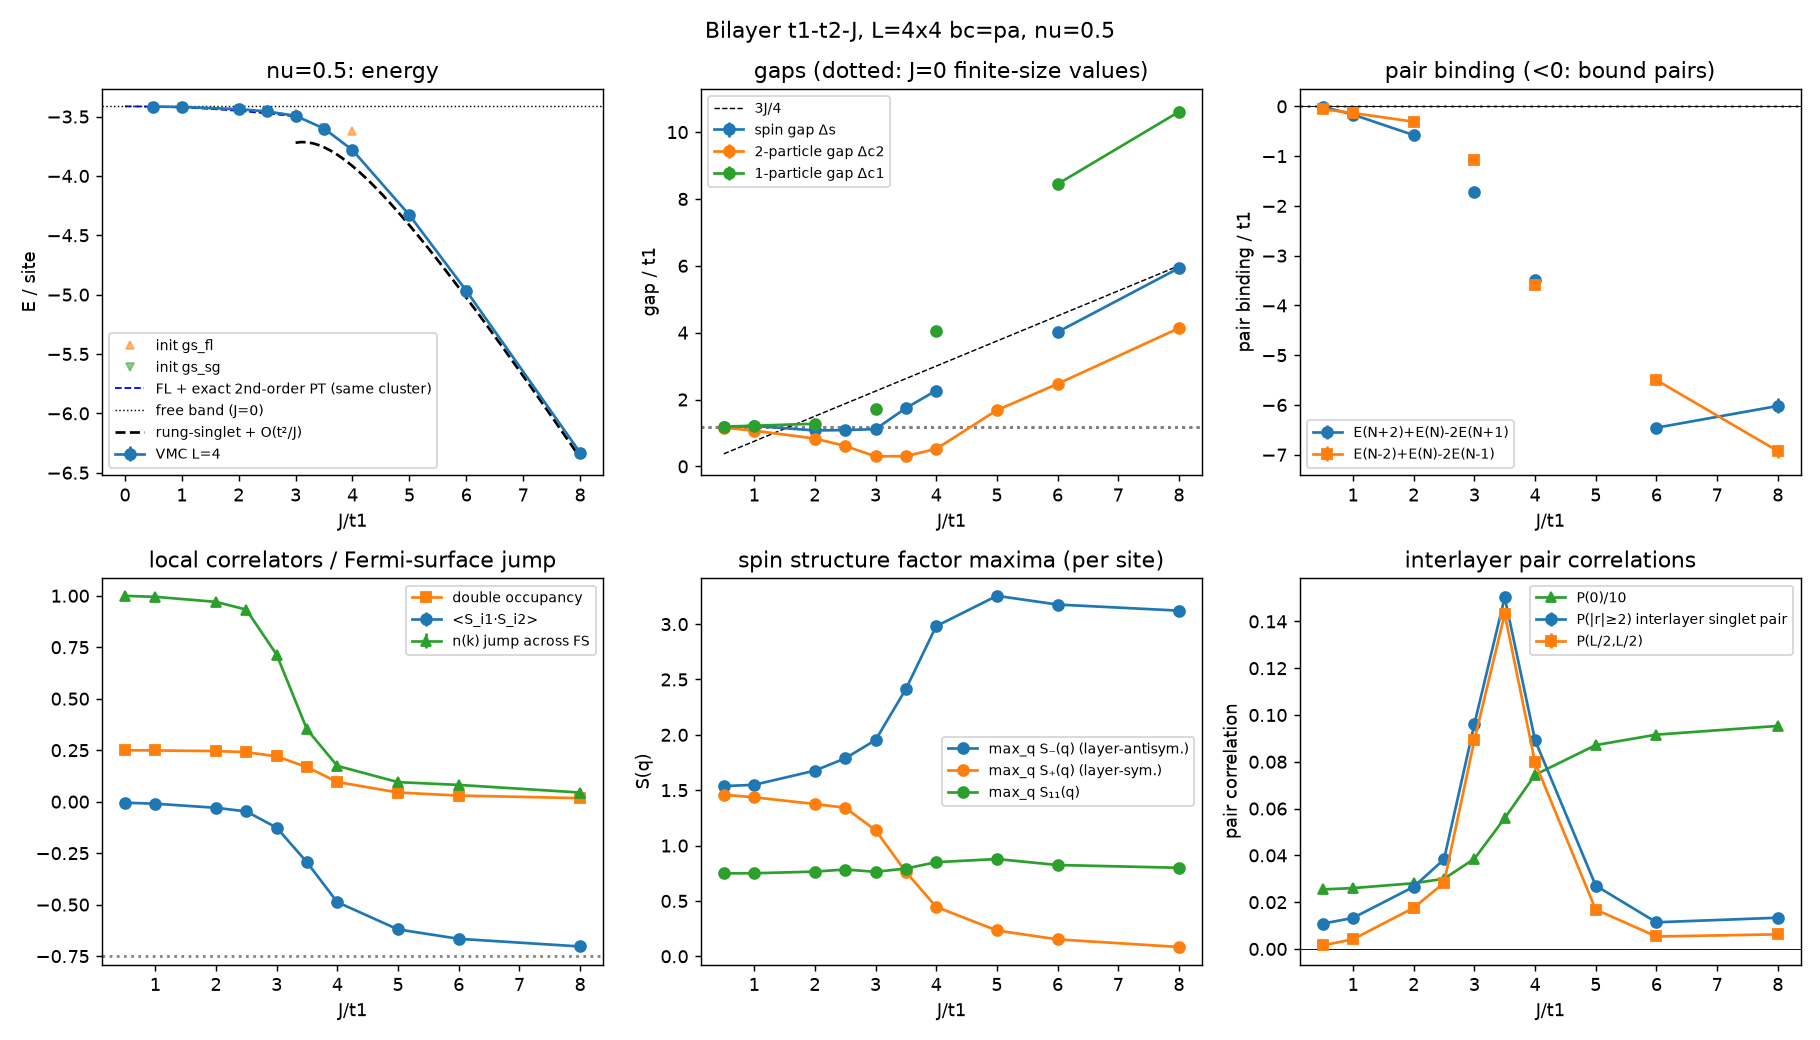
\includegraphics[width=0.95\textwidth]{figures/cut_L4_nu0.500.png}\end{center}

\subsection*{3.2 Weak coupling, J $\le$ 2: Fermi liquid}

The momentum distribution is that of the filled band (n(k) = 1.000/0.000 inside/outside the J = 0 Fermi surface at J = 0.5, 0.998/0.002 at J = 1, 0.98/0.01 at J = 2); the occupied set on this cluster, \{(0,$\pm$$\pi$/4), ($\pm$$\pi$/2,$\pm$$\pi$/4), (0,$\pm$3$\pi$/4)\}, is the Fermi sea of the t$_1$--t$_2$ band, not the nested diamond. All three gaps stay at the one-particle level spacing (1.17 $\pm$ 0.05 at J = 0.5 and 1; at J = 2 the two-particle gap has started to drop, 0.83, and the pair-binding energy to grow, --0.58, the first sign of pairing). The rung spin correlation is --0.005, --0.008, --0.030, two orders of magnitude below the singlet value --3/4; the interlayer pair correlation at distance $\ge$ 2 is at its free-fermion value (0.011--0.027); S$_+$($\pi$,$\pi$) and S$_-$($\pi$,$\pi$) stay at their free values (1.44--1.55) with no peak, and N($\pi$,$\pi$) = 1.47 is the free-fermion value. Energies: the VMC recovers 40--55 \% of the exact second-order correlation energy of this cluster (E$_2$ = --0.0024, --0.0095, --0.0378 per site at J = 0.5, 1, 2), a known limitation of Jastrow-type states at weak coupling; the missing energy is $\le$ 0.02 per site, far below the scale that decides the transitions. Phase label: \textbf{Fermi liquid} (with the caveat of Sec. 3.5 on the exponentially small BCS pairing scale, which is what the J = 2 pair-binding energy is beginning to show).

\subsection*{3.3 Intermediate coupling, J = 3--4: interlayer-singlet superconductor}

Between J = 2 and J = 3 every diagnostic turns over at once. (i) The two optimizations stop agreeing: the state reached from the rung-singlet start is lower by 0.026 (J = 3) and 0.16 (J = 4) per site than the one reached from the Fermi liquid, i.e. the energy landscape has two distinct minima, a Fermi-liquid-like and a paired one, and the paired one wins. (ii) The single-particle gap $\Delta$\_c1 rises above its free value (1.70 at J = 3, 4.06 at J = 4) while the two-particle gap $\Delta$\_c2 \emph{drops below} it (0.30, 0.52 versus 1.17): adding electrons in pairs is cheap, adding them one at a time is expensive. The pair-binding energy E(N+2)+E(N)--2E(N+1) is --1.7 and --3.5: two added electrons bind into an interlayer singlet. (iii) The interlayer singlet pair correlation at the largest distance on the cluster, P(L/2, L/2), jumps from its free-fermion value 0.002--0.018 to 0.089 (J = 3) and 0.080 (J = 4), and the translation-averaged P(|r| $\ge$ 2) to 0.09--0.10, i.e. the pair correlation is essentially distance-independent across the cluster. (iv) n(k) loses its discontinuity (jump 0.71 $\to$ 0.17) and becomes a smooth v\_k$^2$-like profile (0.54 inside / 0.37 outside the free Fermi surface at J = 4). (v) The rung spin correlation grows to --0.13 (J = 3) and --0.49 (J = 4), two thirds of the full singlet value; the layer-symmetric spin structure factor S$_+$($\pi$,$\pi$) collapses (1.46 $\to$ 1.14 $\to$ 0.45 from J = 0.5 to 4) while S$_-$($\pi$,$\pi$) grows (1.54 $\to$ 1.95 $\to$ 2.98) without any sign of a Bragg peak: 2.98 per site is just the value 3 of an uncorrelated rung-singlet product, and the ($\pi$,$\pi$) maximum is broad (\texttt{figures/Sq\_L4\_nu0.500.png}). The rung-density structure factor N($\pi$,$\pi$) decreases (1.47 at J = 1, 0.72 at J = 4): no density order either. (vi) The spin gap stays near the free value at J = 3 (1.11) and rises to 2.27 at J = 4, well below the single-particle gap, so the lowest spin excitation is a bound (rung-triplet-like) pair excitation rather than two free quasiparticles.
\begin{center}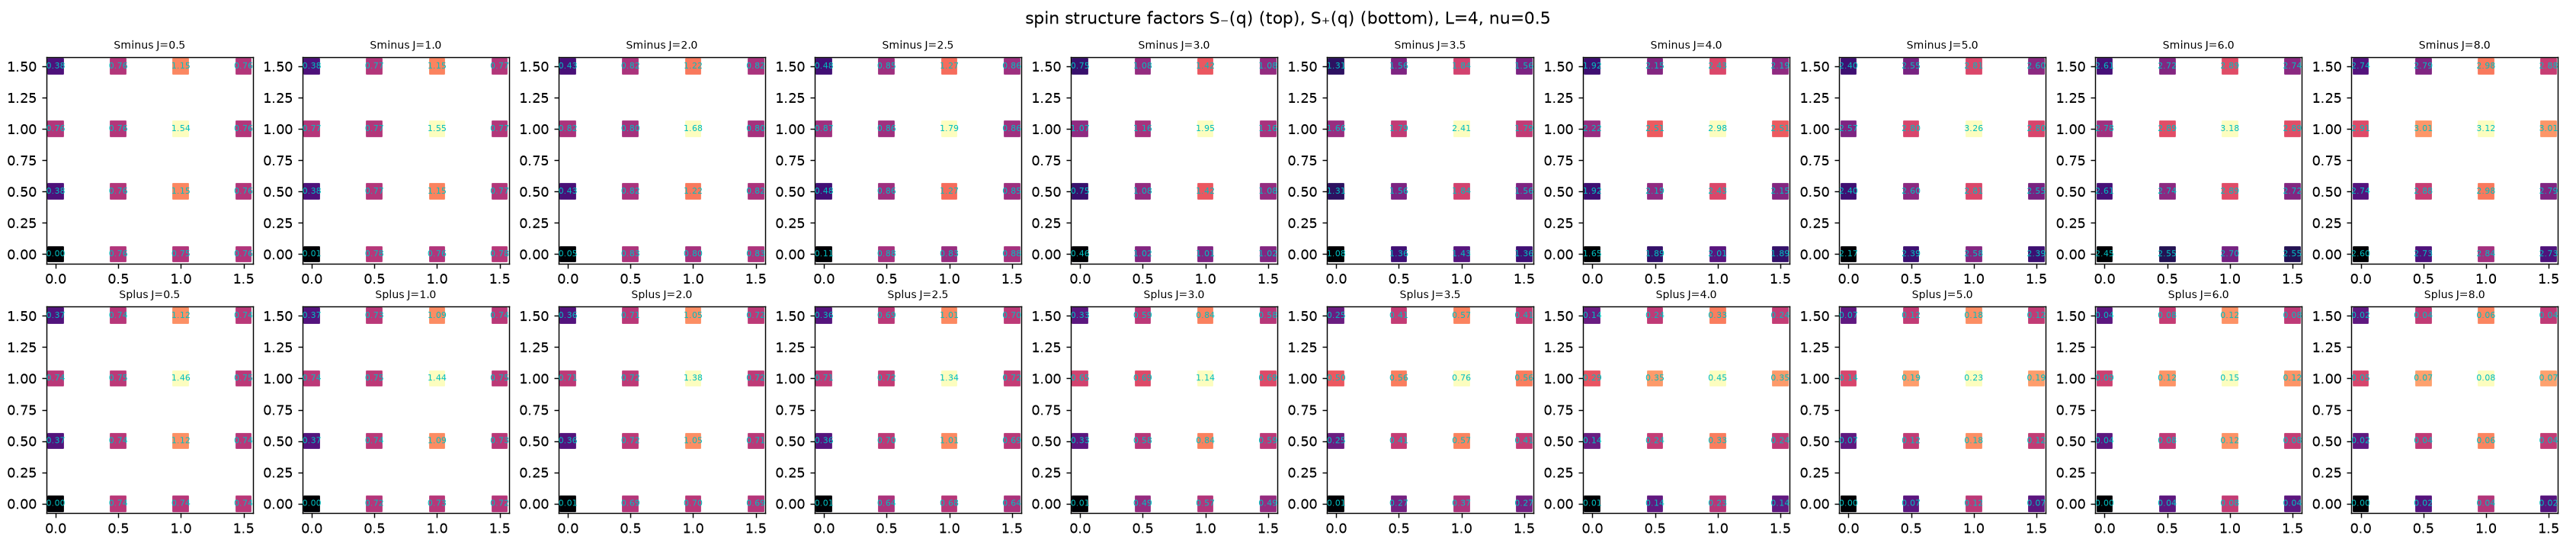
\includegraphics[width=0.95\textwidth]{figures/Sq_L4_nu0.500.png}\end{center}

Taken together: finite single-particle gap, two-particle gap below the finite-size free value, bound pairs, distance-independent pair correlation, no Fermi surface, no magnetic order. Phase label at J = 3 and J = 4: \textbf{superconductor of interlayer singlet pairs}, in the crossover regime between weak-coupling BCS pairing (the mean-field gap at J = 3 is $\Delta$\_BCS $\approx$ 0.49, Sec. 3.5) and the Bose limit of preformed rung singlets. This is not yet the gapped symmetric insulator: the insulator requires the \emph{pair} gap to open, and at J = 4 it is still below the non-interacting finite-size gap.

\subsection*{3.4 Strong coupling, J $\ge$ 6: the symmetric gapped (rung-singlet) insulator}

At J = 6 the picture has reversed: the two-particle gap, which was \emph{below} the free value at J = 3--4, is now 2.47 $\pm$ 0.05 (4.13 $\pm$ 0.07 at J = 8), twice the non-interacting level spacing and consistent with the strong-coupling rung-pair gap 3J/4 minus the pair kinetic energy (1.3 at J = 6 and 3.5 at J = 8 at second order; the variational ground state lies $\approx$ 0.04--0.06 per site above the second-order energy, which inflates all VMC gaps at these J by up to $\approx$ 1); the long-distance pair correlation has fallen back to the free-fermion level (P(L/2,L/2) = 0.005--0.006, from 0.08 at J = 4); n(k) is flat within $\pm$0.1 around 1/2 with no trace of the Fermi surface; the rung correlation is 89 \% (J = 6) and 94 \% (J = 8) of the singlet value and the double occupancy is 0.03 and 0.017; S$_+$($\pi$,$\pi$) (layer-symmetric) is essentially zero (0.15, 0.08) and S$_-$($\pi$,$\pi$) sits at the value 3 of an exact singlet product (3.18, 3.12), a broad maximum rather than a peak that could grow with system size (the 6$\times$6 comparison is in Sec. 3.6); the rung-density structure factor N($\pi$,$\pi$) = 0.14 at J = 8 shows the charge fluctuations frozen out, with no density-wave peak. The spin gap is 4.0 (J = 6) and 5.9 (J = 8), the single-particle gap 8.5 and 10.6, both far larger than the pair gap: single electrons and spin flips must break a singlet, pairs do not. The strong-coupling theory of Sec. 6 gives spin/single/pair gaps 3.05/5.3/1.3 at J = 6 and 5.4/8.0/3.5 at J = 8, the same ordering and magnitudes. Phase label: \textbf{symmetric gapped insulator} (the interlayer-singlet product dressed by hopping, the symmetric-mass-generation state): a charge gap, a spin gap, no magnetic or density Bragg peak, no pair condensate, and every symmetry of H preserved. \textbf{A gapped phase is present on the half-filling cut, for J $\gtrsim$ 5 on the 4$\times$4 lattice.}

\subsection*{3.5 What "Fermi liquid" means on a 4$\times$4 lattice, and where the boundaries are}

The interaction J S\_\{i1\}$\cdot$S\_\{i2\} is attractive in the interlayer singlet pair channel (--3J/4 per singlet), so in mean-field theory the Fermi liquid is unstable to interlayer s-wave pairing at any J > 0 with an exponentially small gap. Solving the BCS gap equation on the infinite lattice at $\nu$ = 1/2 (\texttt{code/bcs\_weak.py}) gives $\Delta$\_BCS = 10$^-$$^4$, 0.007, 0.17, 0.49, 0.87 at J = 0.5, 1, 2, 3, 4. On the 4$\times$4 cluster the one-particle level spacing is 1.17, so pairing is invisible for J $\lesssim$ 2 and sets in between J = 2 and 3, exactly where the VMC diagnostics turn over. The label "Fermi liquid" at J $\le$ 2 therefore means: no pairing resolvable at this lattice size, with a mean-field pairing scale below 0.2; at zero temperature in the thermodynamic limit the weak-coupling state is a superconductor with a gap that is exponentially small in t/J. The Fermi surface at these couplings is the free one of the t$_1$--t$_2$ band, not the nested diamond (t$_2$ removes the nesting; the occupied momenta on the cluster are listed in 3.1), and no interlayer exciton or antiferromagnetic instability appears: S$_+$(q) decreases monotonically with J and S$_-$(q) grows only into the broad rung-singlet form.

Boundaries on the 4$\times$4 cluster, with the extra points J = 2.5, 3.5, 5 included in the table of 3.1: Fermi-liquid-like $\to$ paired superconductor between J = 2.5 (n(k) jump 0.93, P\_pair(r $\ge$ 2) = 0.038, $\Delta$\_c2 = 0.61) and J = 3 (0.71, 0.096, 0.30), i.e. \textbf{J\_c1 $\approx$ 2.7 $\pm$ 0.3}; the pair correlation peaks at J = 3.5 (0.150, n(k) jump 0.35, $\Delta$\_c2 = 0.31, $\Delta$\_s = 1.74). Superconductor $\to$ symmetric gapped insulator between J = 4 ($\Delta$\_c2 = 0.52 below the free value, P\_pair = 0.089) and J = 5 ($\Delta$\_c2 = 1.68 $\pm$ 0.04 above the free value 1.17, P\_pair = 0.027 at the free-fermion level, rung singlet weight 83 \%, S$_+$($\pi$,$\pi$) = 0.23), i.e. \textbf{J\_c2 $\approx$ 4.5 $\pm$ 0.5}. The second-order strong-coupling theory places the closing of the rung-pair gap at J $\approx$ 4.9 (Fig. \texttt{figures/sc\_gaps\_vs\_J.png}), inside that interval, and the BCS estimate puts the resolvable-pairing onset at J $\approx$ 2.5--3. The 6$\times$6 lattice (Sec. 3.6) could not resolve the two-particle gap at J = 4 within the budget; its ground-state correlators put that point close to the superconductor--insulator boundary, so J\_c2 should be read as 4--5 rather than 4.5 $\pm$ 0.5.
\begin{center}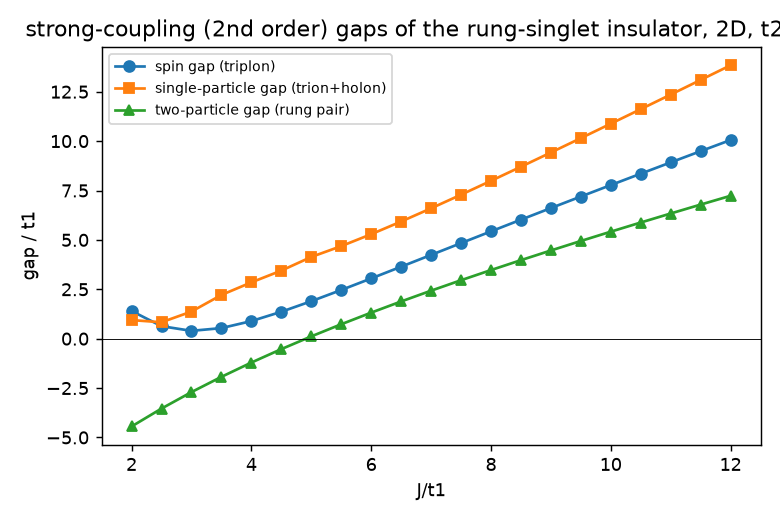
\includegraphics[width=0.95\textwidth]{figures/sc_gaps_vs_J.png}\end{center}


\subsection*{3.6 Finite-size check on the 6$\times$6 bilayer}

6$\times$6 bilayer (144 spin-orbitals, 72 electrons), boundary (P,A), one-particle level gap 0.536 at J = 0; 1024 samples per step. The 6$\times$6 optimization is harder than 4$\times$4: the rung-singlet start produced non-finite steps repeatedly and was abandoned, two BCS-type starts (120 steps, kernel and explicit SR solvers) converged to the same energy --3.61 per site but were not yet at the variational minimum (their N+2 sector, started from them, went 3.1 \emph{below} them, an unambiguous sign of an unconverged ground state). The ground state reported here was therefore re-optimized for a further 150 steps starting from those lower N+2 parameters and reaches --3.7164 $\pm$ 0.0061 per site with R-hat 1.06; its N $\pm$ 2 sectors were then optimized from it for 80 steps. The J = 0 finite-size shift of the free energy between the two clusters is +0.097 per site (--3.317 versus --3.414), so the 6$\times$6 value lies where a converged state should (the 4$\times$4 energy is --3.782).

Comparison of the J = 4 ground states (4$\times$4 $\to$ 6$\times$6): rung correlation --0.488 $\to$ --0.565, double occupancy 0.096 $\to$ 0.065, n(k) jump 0.17 $\to$ 0.05 (both featureless), S$_-$($\pi$,$\pi$) 2.98 $\to$ 3.05 per site (no growth with system size: no magnetic order), S$_+$($\pi$,$\pi$) 0.45 $\to$ 0.34, N($\pi$,$\pi$) 0.72 $\to$ 0.46, interlayer pair correlation at the maximal distance 0.080(3) $\to$ 0.044(4) (free-fermion value $\approx$ 0.002 on 6$\times$6) and translation-averaged P(|r| $\ge$ 2) 0.089 $\to$ 0.051. The pair correlation at J = 4 therefore remains an order of magnitude above the free value on the larger cluster but does not stay constant: it drops by about a factor two while the maximal distance grows from 2$\sqrt{}$2 to 3$\sqrt{}$2 and the rung-singlet weight rises. Two readings are compatible with this: a superconductor whose condensate fraction is smaller than the 4$\times$4 estimate, or a point that lies closer to the superconductor--insulator boundary than the 4$\times$4 labels suggest, i.e. J\_c2 nearer 4 than 4.5. The two-particle gap on 6$\times$6 decides between them: in the superconductor it must fall well below the 4$\times$4 value 0.52 (the finite-size pair gap of a condensate scales as 1/N), in the insulator it must stay of order the 4$\times$4 value or grow.

\textbf{Outcome of the 6$\times$6 gap: inconclusive.} Energies obtained (total, 6$\times$6, J = 4): N sector --133.79 $\pm$ 0.22 (re-optimized), N+2: --133.42 $\pm$ 0.16 (first round, 80 steps from the first ground state) and --129.22 $\pm$ 0.31 (second round, 80 steps from the re-optimized ground state); N--2: --131.17 $\pm$ 0.27 (first round) and --134.32 $\pm$ 0.14 (second round). The two-particle gap is therefore 2.02 $\pm$ 0.28 if the second-round sectors are used and --0.08 $\pm$ 0.25 if the lowest energy of each sector is used; a negative value is impossible for exact energies, so the sector optimizations are mutually inconsistent at the level of $\approx$ 2--4 in total energy (0.05--0.1 per site), which is larger than the gap being measured. The table below lists the second-round numbers for completeness. What the 6$\times$6 calculation does establish is the ground-state comparison above: at J = 4 the 6$\times$6 state has a rung-singlet weight of 75 \% (65 \% on 4$\times$4), its pair correlation at the maximal distance is still twenty times the free-fermion value but half the 4$\times$4 value, and no spin or charge structure-factor peak grows with the cluster. The J = 4 point is therefore near the superconductor--insulator boundary, which on larger lattices may lie somewhat below the 4$\times$4 estimate J\_c2 $\approx$ 4.5 (the second-order strong-coupling estimate is 4.9, the 6$\times$6 ground-state correlators would be consistent with a value closer to 4). Settling it needs sector energies converged to $\approx$ 0.01 per site on 6$\times$6, i.e. several hundred optimization steps per sector, which did not fit the time budget (each 6$\times$6 step costs $\approx$ 60 s on 8 CPU cores; the same step takes 3.2 s on one H200 GPU with chunked local energies, see Section 8, so the missing sector runs are a few GPU-hours rather than a CPU-day).

Energies and gaps, 6x6 bilayer, bc=pa, nu=0.5. Free-band (J=0) references: spin gap 0.536, 2-particle gap 0.536, 1-particle gap 0.536.

\begin{center}\footnotesize\setlength{\tabcolsep}{3pt}
\resizebox{\textwidth}{!}{%
\begin{tabular}{llllllll}\toprule
J & E/site & init (split) & $\Delta$\_s & $\Delta$\_c2 & $\Delta$\_c1 & E\_pb(+) & E\_pb(--) \\ \midrule
4 & -3.7164(61) & bcs & --- & 2.02(28) & --- & --- & --- \\
\bottomrule\end{tabular}}\end{center}

Correlation diagnostics (per site):

\begin{center}\footnotesize\setlength{\tabcolsep}{3pt}
\resizebox{\textwidth}{!}{%
\begin{tabular}{lllllllllll}\toprule
J & $\langle$S\_i1$\cdot$S\_i2$\rangle$ & double occ. & n(k) jump & n(k) in/out & S$_-$($\pi$,$\pi$) & S$_+$($\pi$,$\pi$) & N($\pi$,$\pi$) & P\_pair(r$\ge$2) & P\_pair(L/2,L/2) & P\_pair(0) \\ \midrule
4 & -0.5645(70) & 0.0651(27) & 0.0530(88) & 0.48/0.43 & 3.052(41) & 0.336(41) & 0.46 & 0.0511(11) & 0.0438(43) & 0.8188(69) \\
\bottomrule\end{tabular}}\end{center}

\section*{4. Quarter-filling cut ($\nu$ = 1/4)}

Lattice 4$\times$4 bilayer, boundary (A,A), N = 16 electrons (8 per layer, 4 per layer per spin), closed shell at J = 0 with a one-particle level gap of 3.628 (the four lowest levels at $\varepsilon$ = --3.23 are filled, the next eight at +0.40 are empty); this large finite-size gap is the reference for every gap below and, as discussed in 4.3, it delays the onset of resolvable pairing on this cluster. Free-band energy --3.22843 per site; exact second-order energy E$_2$ = --0.0009, --0.0036, --0.0142 per site at J = 0.5, 1, 2.

\subsection*{4.1 Results along the cut}

Energies and gaps, 4x4 bilayer, bc=aa, nu=0.25. Free-band (J=0) references: spin gap 3.628, 2-particle gap 3.628, 1-particle gap 3.628.

\begin{center}\footnotesize\setlength{\tabcolsep}{3pt}
\resizebox{\textwidth}{!}{%
\begin{tabular}{llllllll}\toprule
J & E/site & init (split) & $\Delta$\_s & $\Delta$\_c2 & $\Delta$\_c1 & E\_pb(+) & E\_pb(--) \\ \midrule
0.5 & -3.228727(10) & fl (0.0000) & 3.62759(33) & 3.5112(12) & 3.62893(45) & -0.1381(23) & -0.0974(11) \\
1 & -3.229779(24) & sg (0.0002) & 3.6007(30) & 3.3210(25) & 3.6442(69) & -0.437(14) & -0.2092(37) \\
2 & -3.23414(16) & sg (0.0007) & 3.6351(69) & 2.9239(63) & 3.665(14) & -0.980(27) & -0.5017(80) \\
2.5 & -3.2400(10) & sg (0.0049) & 3.498(20) & 2.730(18) & --- & --- & --- \\
3 & -3.2452(11) & sg (0.0024) & 3.647(23) & 2.469(19) & 3.552(38) & -1.426(29) & -0.740(28) \\
4 & -3.2746(14) & fl (0.0054) & 3.666(29) & 1.956(27) & 3.858(50) & -2.493(46) & -1.313(39) \\
5 & -3.3189(19) & sg (0.0078) & 3.716(40) & 1.322(35) & --- & --- & --- \\
6 & -3.4149(22) & fl (0.0010) & 3.931(45) & 0.381(38) & 4.480(79) & -5.115(67) & -3.083(60) \\
8 & -3.8683(17) & fl (0.0001) & 5.296(36) & 0.228(30) & 5.919(61) & -6.253(61) & -5.127(49) \\
\bottomrule\end{tabular}}\end{center}

Correlation diagnostics (per site):

\begin{center}\footnotesize\setlength{\tabcolsep}{3pt}
\resizebox{\textwidth}{!}{%
\begin{tabular}{lllllllllll}\toprule
J & $\langle$S\_i1$\cdot$S\_i2$\rangle$ & double occ. & n(k) jump & n(k) in/out & S$_-$($\pi$,$\pi$) & S$_+$($\pi$,$\pi$) & N($\pi$,$\pi$) & P\_pair(r$\ge$2) & P\_pair(L/2,L/2) & P\_pair(0) \\ \midrule
0.5 & -0.00089(33) & 0.06243(58) & 1.00 & 1.00/0.00 & 0.7515(37) & 0.7438(37) & 1.01 & 0.000349(94) & 0.00052(22) & 0.06375(41) \\
1 & -0.00243(26) & 0.06284(57) & 1.00 & 1.00/0.00 & 0.7580(37) & 0.7440(37) & 0.99 & 0.000261(100) & 0.00025(24) & 0.06558(37) \\
2 & -0.00569(40) & 0.06283(56) & 0.99808(11) & 1.00/0.00 & 0.7554(40) & 0.7367(40) & 1.01 & 0.00105(14) & 0.00091(29) & 0.06815(48) \\
2.5 & -0.01195(85) & 0.06198(58) & 0.99350(25) & 1.00/0.00 & 0.7656(48) & 0.7244(48) & 1.06 & 0.00703(25) & 0.00688(62) & 0.07498(93) \\
3 & -0.01842(81) & 0.05964(56) & 0.98680(35) & 0.99/0.00 & 0.7835(50) & 0.7200(50) & 0.99 & 0.01213(35) & 0.01157(90) & 0.08197(90) \\
4 & -0.02885(86) & 0.05859(45) & 0.97578(49) & 0.98/0.01 & 0.8061(52) & 0.7076(52) & 0.98 & 0.01761(33) & 0.01672(83) & 0.09356(94) \\
5 & -0.0565(12) & 0.05160(57) & 0.93232(84) & 0.95/0.02 & 0.8879(56) & 0.6556(56) & 1.04 & 0.03925(44) & 0.0372(11) & 0.1251(14) \\
6 & -0.1628(16) & 0.03026(41) & 0.7166(16) & 0.80/0.08 & 1.0447(61) & 0.4859(61) & 1.18 & 0.11788(55) & 0.1149(14) & 0.2463(18) \\
8 & -0.2685(15) & 0.01076(35) & 0.4666(23) & 0.62/0.16 & 1.2560(74) & 0.2956(74) & 1.52 & 0.17255(75) & 0.1673(23) & 0.3685(17) \\
\bottomrule\end{tabular}}\end{center}

Figures: \texttt{figures/cut\_L4\_nu0.250.png}, \texttt{figures/nk\_L4\_nu0.250.png}, \texttt{figures/Sq\_L4\_nu0.250.png}.
\begin{center}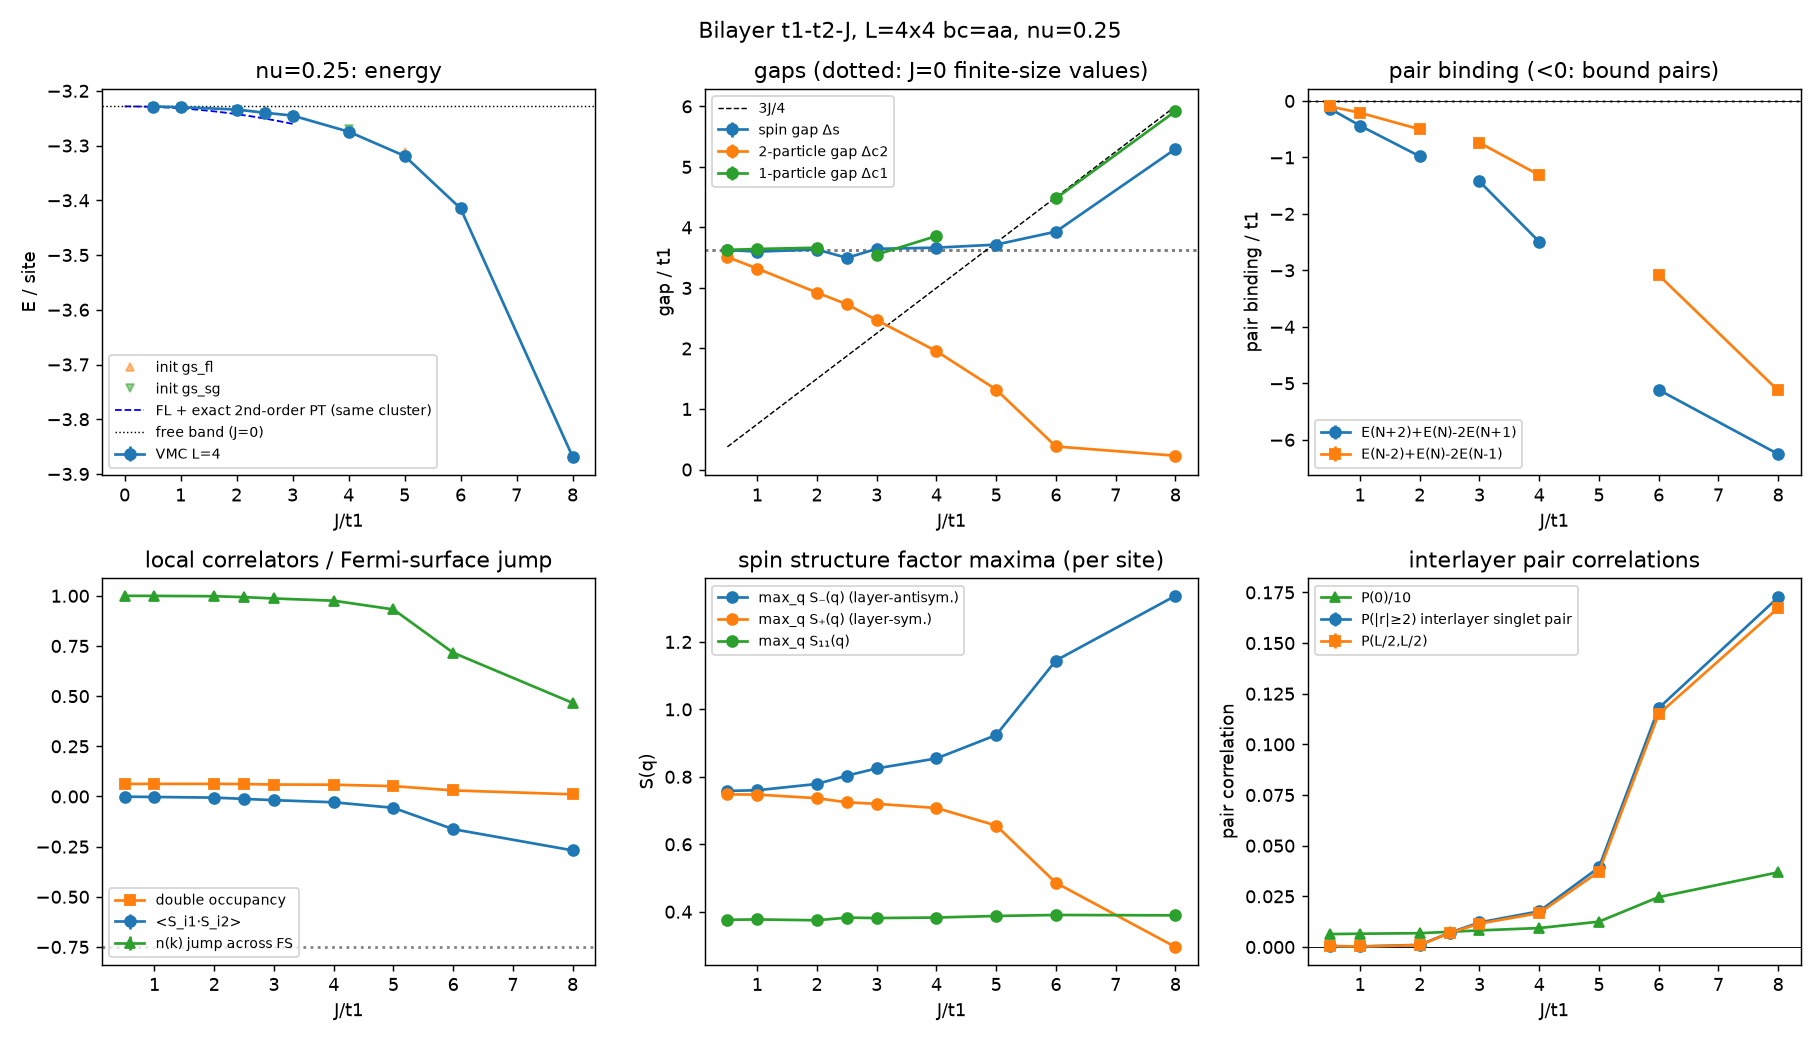
\includegraphics[width=0.95\textwidth]{figures/cut_L4_nu0.250.png}\end{center}

\subsection*{4.2 Weak and intermediate coupling, J $\le$ 5: Fermi liquid with bound added pairs}

For J $\le$ 5 the ground state is the free Fermi sea: n(k) = 1.00/0.00 on the occupied/empty levels up to J = 3, 0.98/0.01 at J = 4 and 0.95/0.02 at J = 5 (the Fermi surface is the small pocket around (0,0) of the t$_1$--t$_2$ band: occupied momenta ($\pm$$\pi$/4, $\pm$$\pi$/4)); the single-particle gap stays at the level spacing (3.55--3.86 versus 3.63) and so does the spin gap (3.60--3.67); the rung spin correlation is $\le$ 0.03 in magnitude; the interlayer pair correlation at distance $\ge$ 2 is $\le$ 0.04; S$_+$($\pi$,$\pi$), S$_-$($\pi$,$\pi$) and N($\pi$,$\pi$) are at their free values (0.7--0.9 and $\approx$ 1.0). The two optimizations agree to $\le$ 0.008 per site. The one quantity that moves is the two-particle sector: $\Delta$\_c2 falls from 3.51 (J = 0.5) to 1.96 (J = 4) and 1.32 (J = 5), and the pair-binding energy E(N+2)+E(N)--2E(N+1) grows to --2.5 at J = 4: two electrons \emph{added} to the quarter-filled Fermi sea bind into an interlayer singlet long before the Fermi sea itself pairs. On this cluster the ground state remains unpaired because the closed-shell gap 3.63 exceeds the pairing scale. Phase label: \textbf{Fermi liquid} for J $\le$ 5 at this lattice size (see 4.4 for the thermodynamic-limit caveat).

\subsection*{4.3 Strong coupling, J = 6--8: superconductor of rung pairs, not a pair crystal}

At J = 6 the ground state has paired: the two-particle gap collapses to 0.38 $\pm$ 0.04 (0.23 at J = 8), far below the free value 3.63, while the single-particle gap rises to 4.5 and 5.9; the pair-binding energy is --5.1 and --6.3; the interlayer pair correlation at the largest distance is 0.115 (J = 6) and 0.167 (J = 8), equal to the translation-averaged value at |r| $\ge$ 2, i.e. distance independent (the free value is 0.0005); n(k) is smeared (jump 0.72 $\to$ 0.47); the rung singlet weight is 22 \% and 36 \% (the maximum for one pair per two rungs is 50 \%); the double occupancy drops to 0.011. The rung-density structure factor N($\pi$,$\pi$) is 1.18 (J = 6) and 1.52 (J = 8) against the free value 1.0: a mild enhancement, an order of magnitude below the value 16 that a checkerboard crystal of rung pairs (two electrons on every other rung) would give on this cluster. The spin gap stays large (3.93 at J = 6, 5.30 at J = 8): every electron is paired and a spin flip must break a pair. Phase label: \textbf{superconductor of interlayer singlet (rung) pairs}, in its Bose-condensate regime: at J = 8 the system is a superfluid of charge-2e rung pairs at pair density 1/2 per site, with no density-wave order. This is the doped counterpart of the insulator of Sec. 3: the same rung pairs that form a Mott insulator at one pair per site are mobile at half a pair per site, with effective hopping t\_b $\approx$ 8t$^2$/3J and nearest-neighbour repulsion V $\approx$ 1.4 t\_b (Sec. 6), below the threshold V/t\_b $\approx$ 2 for a checkerboard crystal; the VMC confirms the superfluid.

\subsection*{4.4 Where the boundary is, and the caveat}

On the 4$\times$4 cluster the Fermi liquid $\to$ superconductor change happens between J = 5 (n(k) jump 0.93, P\_pair(r $\ge$ 2) = 0.039, $\Delta$\_c2 = 1.32 still above the pair-binding scale, rung correlation --0.06) and J = 6 (0.72, 0.118, 0.38, --0.16), i.e. J\_c $\approx$ 5.5 $\pm$ 0.5 on this cluster, about twice the half-filling value. The weak-coupling BCS estimate for $\nu$ = 1/4 (Sec. 3.5) gives $\Delta$\_BCS = 0.015, 0.14, 0.43 at J = 2, 3, 4, i.e. the thermodynamic-limit state is already a weak superconductor at J $\approx$ 3--4; the cluster's level spacing (3.63) hides this, which is why the pair-binding energy, a two-particle quantity with no such threshold, turns on first. The honest statement is: resolvable pairing on 4$\times$4 for J $\ge$ 6; mean-field pairing scale above 0.1 for J $\gtrsim$ 3; no resolvable pairing and a free Fermi sea for J $\le$ 2 at any size.

\section*{5. Phase diagram in the ($\nu$, J) plane}

\subsection*{5.1 How a point is labelled}

Each grid point is labelled from the same finite-size diagnostics as the line cuts, always relative to the exact J = 0 values of the same cluster and boundary condition:

\begin{itemize}
\item \textbf{Fermi liquid}: n(k) jump across the J = 0 Fermi surface > 0.9, two-particle gap within 0.3 of its free
value, no pair correlation beyond a few times the free-fermion value, no Bragg peak in S(q).
\item \textbf{Superconductor (interlayer singlet pairs)}: long-distance interlayer pair correlation P(|r| $\ge$ 2) $\ge$ 0.05 per
site (free value 0.0005--0.01), n(k) smeared (jump < 0.9), two-particle gap not above its free value by more
than 0.5; the pair-binding energy E(N+2) + E(N) -- 2E(N+1) is negative and the single-particle gap exceeds the
pair gap at every such point.
\item \textbf{Symmetric gapped (SMG) insulator}: two-particle and single-particle gaps both exceed their free values by
more than 0.5, n(k) featureless (jump < 0.35), no long-range pair correlation (< 0.03), no Bragg peak.
\item \textbf{Magnetic / density order}: a peak of S$_-$(q), S$_+$(q) or N(q) that grows with lattice size (checked with 6$\times$6
at half filling only).
\item \textbf{Crossover}: none of the above holds cleanly.
\end{itemize}
The thresholds are stated so the labels are reproducible from \texttt{data/summary.json} (\texttt{code/plot\_phase\_diagram.py}); they are finite-size operational criteria, not a claim that a crossover point is a distinct phase.

\subsection*{5.2 Symmetry $\nu$ $\to$ 1 -- $\nu$}

Under the particle-hole transformation c\_\{i$\ell$$\sigma$\} $\to$ (--1)\^{}\{i\} c$^\dagger$\_\{i$\ell$$\sigma$\} the exchange term is invariant and t$_1$ $\to$ --t$_1$ (a gauge choice), but t$_2$ $\to$ --t$_2$. The phase diagram is therefore symmetric about $\nu$ = 1/2 only up to the sign of t$_2$; with t$_2$ = 0.2 the two halves are related by t$_2$ $\leftrightarrow$ --t$_2$, which moves the van Hove singularity and changes the Fermi-surface shape but not the strong-coupling (rung-pair) physics. The grid below is computed for $\nu$ $\le$ 3/4 plus a check row at $\nu$ = 5/8 to measure the asymmetry directly rather than assuming it away.


\subsection*{5.3 Results on the ($\nu$, J) grid}

\begin{center}\footnotesize\setlength{\tabcolsep}{3pt}
\resizebox{\textwidth}{!}{%
\begin{tabular}{lllllllllllll}\toprule
$\nu$ & bc & J & E/site & $\Delta$\_c2 -- $\Delta$\_c2(J=0) & $\Delta$\_c1 -- $\Delta$\_c1(J=0) & E\_pb & $\langle$S\_i1$\cdot$S\_i2$\rangle$ & n(k) jump & P\_pair(r$\ge$2) & S$_-$($\pi$,$\pi$) & N($\pi$,$\pi$) & label \\ \midrule
0.125 & pa & 1 & -1.9904 & -0.16 & --- & --- & -0.001 & 1.00 & 0.005 & 0.37 & 0.53 & FL \\
0.125 & pa & 2 & -1.9916 & -0.31 & --- & --- & -0.001 & 1.00 & 0.005 & 0.38 & 0.50 & FL \\
0.125 & pa & 3 & -1.9998 & -0.56 & --- & --- & -0.007 & 0.99 & 0.010 & 0.38 & 0.51 & FL \\
0.125 & pa & 4 & -2.0094 & -0.87 & --- & --- & -0.012 & 0.98 & 0.015 & 0.39 & 0.51 & FL \\
0.125 & pa & 6 & -2.0561 & -1.67 & --- & --- & -0.041 & 0.86 & 0.041 & 0.42 & 0.55 & crossover \\
0.125 & pa & 8 & -2.1942 & -2.20 & --- & --- & -0.097 & 0.58 & 0.090 & 0.53 & 0.69 & SC (interlayer pairs) \\
0.250 & aa & 0.5 & -3.2287 & -0.12 & 0.00 & -0.14 & -0.001 & 1.00 & 0.000 & 0.75 & 1.01 & FL \\
0.250 & aa & 1 & -3.2298 & -0.31 & 0.02 & -0.44 & -0.002 & 1.00 & 0.000 & 0.76 & 0.99 & FL \\
0.250 & aa & 2 & -3.2341 & -0.70 & 0.04 & -0.98 & -0.006 & 1.00 & 0.001 & 0.76 & 1.01 & FL \\
0.250 & aa & 2.5 & -3.2400 & -0.90 & --- & --- & -0.012 & 0.99 & 0.007 & 0.77 & 1.06 & FL \\
0.250 & aa & 3 & -3.2452 & -1.16 & -0.08 & -1.43 & -0.018 & 0.99 & 0.012 & 0.78 & 0.99 & FL \\
0.250 & aa & 4 & -3.2746 & -1.67 & 0.23 & -2.49 & -0.029 & 0.98 & 0.018 & 0.81 & 0.98 & FL \\
0.250 & aa & 5 & -3.3189 & -2.31 & --- & --- & -0.057 & 0.93 & 0.039 & 0.89 & 1.04 & FL \\
0.250 & aa & 6 & -3.4149 & -3.25 & 0.85 & -5.12 & -0.163 & 0.72 & 0.118 & 1.04 & 1.18 & SC (interlayer pairs) \\
0.250 & aa & 8 & -3.8683 & -3.40 & 2.29 & -6.25 & -0.269 & 0.47 & 0.173 & 1.26 & 1.52 & SC (interlayer pairs) \\
0.375 & pa & 1 & -3.4064 & -0.08 & --- & --- & -0.006 & 1.00 & 0.007 & 1.16 & 1.55 & FL \\
0.375 & pa & 2 & -3.4227 & -0.35 & --- & --- & -0.022 & 0.98 & 0.017 & 1.20 & 1.49 & FL \\
0.375 & pa & 3 & -3.4587 & -0.75 & --- & --- & -0.049 & 0.94 & 0.035 & 1.29 & 1.41 & FL \\
0.375 & pa & 4 & -3.5865 & -1.25 & --- & --- & -0.235 & 0.48 & 0.151 & 1.68 & 1.34 & SC (interlayer pairs) \\
0.375 & pa & 6 & -4.2853 & -1.24 & --- & --- & -0.423 & 0.20 & 0.177 & 2.12 & 1.08 & SC (interlayer pairs) \\
0.375 & pa & 8 & -5.1932 & -1.31 & --- & --- & -0.478 & 0.14 & 0.172 & 2.17 & 0.99 & SC (interlayer pairs) \\
0.500 & pa & 0.5 & -3.4155 & -0.01 & 0.02 & -0.01 & -0.005 & 1.00 & 0.011 & 1.54 & 1.97 & FL \\
0.500 & pa & 1 & -3.4190 & -0.10 & 0.04 & -0.16 & -0.010 & 0.99 & 0.013 & 1.55 & 1.47 & FL \\
0.500 & pa & 2 & -3.4375 & -0.34 & 0.10 & -0.58 & -0.030 & 0.97 & 0.027 & 1.68 & 1.95 & FL \\
0.500 & pa & 2.5 & -3.4567 & -0.56 & --- & --- & -0.047 & 0.93 & 0.038 & 1.79 & --- & FL \\
0.500 & pa & 3 & -3.4936 & -0.87 & 0.53 & -1.73 & -0.126 & 0.71 & 0.096 & 1.95 & 1.69 & SC (interlayer pairs) \\
0.500 & pa & 3.5 & -3.6008 & -0.87 & --- & --- & -0.294 & 0.35 & 0.150 & 2.41 & --- & SC (interlayer pairs) \\
0.500 & pa & 4 & -3.7821 & -0.65 & 2.88 & -3.49 & -0.488 & 0.17 & 0.089 & 2.98 & 0.72 & SC (interlayer pairs) \\
0.500 & pa & 5 & -4.3294 & 0.51 & --- & --- & -0.620 & 0.09 & 0.027 & 3.26 & --- & SMG insulator \\
0.500 & pa & 6 & -4.9667 & 1.30 & 7.27 & -6.46 & -0.666 & 0.08 & 0.011 & 3.18 & 0.22 & SMG insulator \\
0.500 & pa & 8 & -6.3298 & 2.96 & 9.44 & -6.02 & -0.703 & 0.04 & 0.013 & 3.12 & 0.14 & SMG insulator \\
0.625 & pa & 4 & -3.3816 & -0.07 & --- & --- & -0.339 & 0.05 & 0.171 & 1.89 & 1.27 & SC (interlayer pairs) \\
0.625 & pa & 8 & -5.1551 & -0.11 & --- & --- & -0.495 & 0.01 & 0.162 & 2.12 & 0.94 & SC (interlayer pairs) \\
0.750 & aa & 1 & -2.4304 & -0.32 & --- & --- & -0.004 & 1.00 & 0.002 & 0.76 & 1.01 & FL \\
0.750 & aa & 2 & -2.4428 & -0.72 & --- & --- & -0.017 & 0.99 & 0.011 & 0.79 & 1.02 & FL \\
0.750 & aa & 3 & -2.4731 & -1.35 & --- & --- & -0.051 & 0.93 & 0.038 & 0.83 & 1.04 & FL \\
0.750 & aa & 4 & -2.5891 & -1.82 & --- & --- & -0.184 & 0.63 & 0.130 & 1.05 & 1.32 & SC (interlayer pairs) \\
0.750 & aa & 6 & -3.0763 & -1.84 & --- & --- & -0.282 & 0.36 & 0.171 & 1.23 & 1.69 & SC (interlayer pairs) \\
0.750 & aa & 8 & -3.6723 & -1.92 & --- & --- & -0.315 & 0.26 & 0.178 & 1.32 & 1.85 & SC (interlayer pairs) \\
0.875 & pa & 2 & -1.4317 & -0.42 & --- & --- & -0.010 & 0.98 & 0.013 & 0.38 & 0.51 & FL \\
0.875 & pa & 8 & -1.9515 & -1.32 & --- & --- & -0.146 & 0.25 & 0.129 & 0.61 & 0.81 & SC (interlayer pairs) \\
\bottomrule\end{tabular}}\end{center}

The figure \texttt{figures/phase\_diagram\_L4.png} shows the labels on the plane with the two cuts marked. Boundary conditions per filling are the closed-shell choices of Sec. 2.4; the J = 0 level gap that every finite-size gap is measured against is 2.57 ($\nu$ = 1/8), 3.63 (1/4), 1.39 (3/8), 1.17 (1/2), 0.26 (5/8), 2.03 (3/4), 1.43 (7/8).
\begin{center}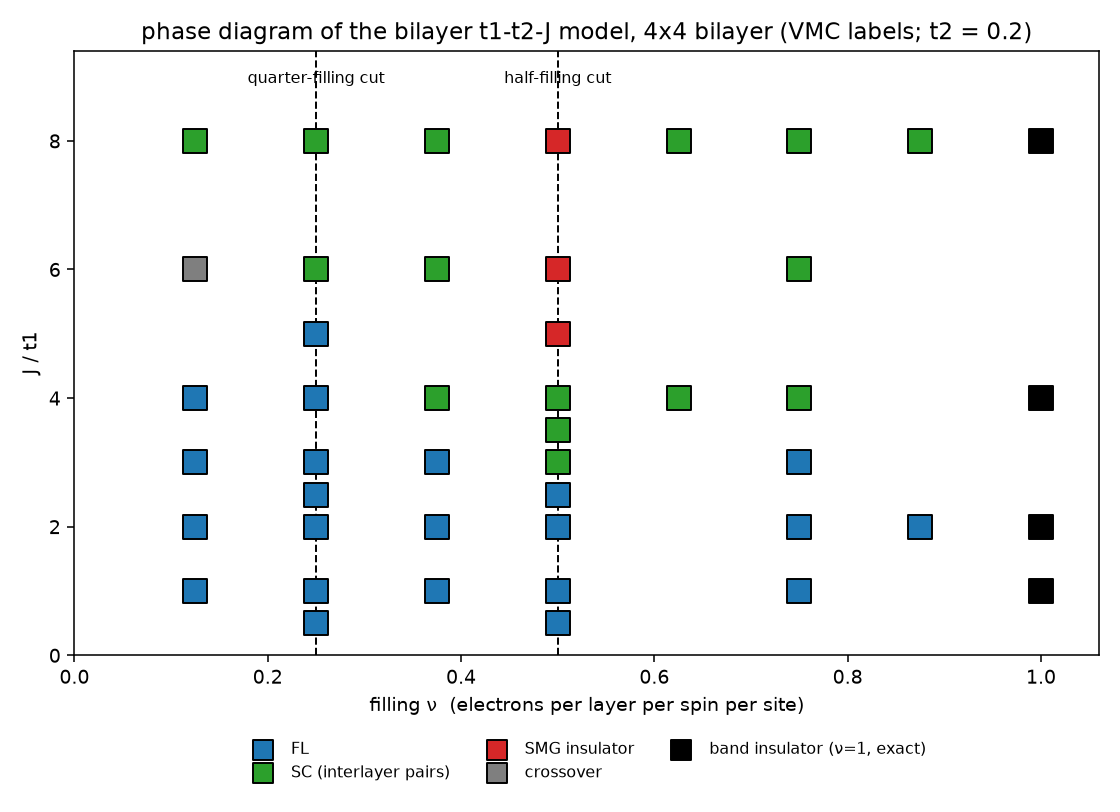
\includegraphics[width=0.95\textwidth]{figures/phase_diagram_L4.png}\end{center}

Reading of the plane:

\begin{itemize}
\item \textbf{The symmetric gapped insulator exists only on the half-filling line.} At every filling $\nu$ $\ne$ 1/2, including
$\nu$ = 3/8 and 5/8 next to it, the two-particle gap stays \emph{below} its free value up to J = 8 and the long-range
pair correlation stays at 0.13--0.17 per site: the rung pairs that are frozen at one per site at $\nu$ = 1/2 are
mobile as soon as the density moves. The insulator is filling-enforced.
\item \textbf{A superconducting region of rung (interlayer singlet) pairs surrounds it.} It covers every filling at large
J (J = 8 at all six fillings) and extends down to J = 4 at $\nu$ = 3/8, 5/8 and 3/4 ($\nu$ = 3/8 is still a Fermi
liquid at J = 3) and to J = 3 at $\nu$ = 1/2; its lower boundary in J rises as the density moves away from half
filling (J $\approx$ 5 at $\nu$ = 1/4; at $\nu$ = 1/8 the point J = 6 is the crossover itself, with n(k) jump 0.86 and
P\_pair(r $\ge$ 2) = 0.041, and J = 8 is paired), tracking the smaller density of states and the larger level
spacing of the dilute pockets. No
density-wave peak appears anywhere (N($\pi$,$\pi$) $\le$ 1.8, versus $\ge$ 10 for a pair crystal on this cluster).
\item \textbf{The Fermi liquid occupies the weak-coupling corner at every filling}, with the caveat that its true
thermodynamic-limit fate at any J > 0 is a superconductor with an exponentially small gap (Sec. 3.5); the
boundary drawn here is where pairing becomes resolvable on 4$\times$4.
\item \textbf{Particle--hole symmetry.} $\nu$ = 3/8 and 5/8, $\nu$ = 1/4 and 3/4, and $\nu$ = 1/8 and 7/8 carry the same labels at the
same J ($\nu$ = 7/8: Fermi liquid at J = 2, rung-pair superconductor at J = 8 with P\_pair(r $\ge$ 2) = 0.129); the
quantitative differences (e.g. at J = 4: P\_pair(r $\ge$ 2) = 0.151 at $\nu$ = 3/8 versus 0.171 at 5/8, rung correlation
--0.235 versus --0.339) reflect the t$_2$ $\to$ --t$_2$ asymmetry and, more strongly, the different level spacings of the
two closed-shell clusters (1.39 versus 0.26). The plane is symmetric about $\nu$ = 1/2 in its phases, not in its
numbers. $\nu$ = 1 is the trivial band insulator (E = 0 exactly, every mode filled), computed analytically.
\item \textbf{Magnetism.} S$_-$($\pi$,$\pi$) grows with J at every filling but saturates at the value of an uncorrelated product
of rung singlets (3 per site at $\nu$ = 1/2, proportionally less at the other fillings) and S$_+$($\pi$,$\pi$) decreases; no
peak that could become a Bragg peak is found at any ($\nu$, J). The t$_2$ = 0.2 band has no nesting-driven instability at these
couplings.
\end{itemize}

\section*{6. Spectra of the gapped phase at half filling}

\subsection*{6.1 Approximation used, and how it is tied to the variational state}

None of the three requested spectra is a ground-state expectation value, so an explicit approximation is needed. I use the \textbf{strong-coupling quasiparticle theory of the rung-singlet state}, with every effective amplitude extracted \emph{exactly} from the diagonalization of two rungs joined by one bond (\texttt{code/strong\_coupling.py}) and combined by bond additivity, which is exact to first order in t for charge excitations and to second order (t$^2$/J) for spin excitations and diagonal shifts. The variational state of Section 3 at the chosen J is the same rung-singlet product dressed by hopping (its rung correlation $\langle$S\_\{i1\}$\cdot$S\_\{i2\}$\rangle$ and the pairing function are reported there), and the VMC gaps are compared with the theory's gaps at the same J; agreement of the gaps is the check that the excitation picture matches the variational ground state.

Excitations of the rung-singlet background and their bands (amplitudes per bond from two-rung ED; signs from the parity of the lowest two-rung level):

\begin{itemize}
\item \textbf{Trion} (three-electron rung, electron addition) and \textbf{holon} (one-electron rung, electron removal):
$\varepsilon$(k) = e$_0$ + 2a$_1$(cos k\_x + cos k\_y) + 2a$_2$[cos(k\_x+k\_y) + cos(k\_x--k\_y)]. The hopping a$_1$ $\to$ t/2 at large J
(0.378 at J=8): the quasiparticle keeps its spin and layer and moves with half the bare amplitude because the
singlet on the rung it enters has overlap 1/$\sqrt{}$2 with the product it leaves behind. The trion band minimum is at
k=0 and the holon band minimum at ($\pi$,$\pi$).
\item \textbf{Triplon} (rung triplet, S=1): $\omega$(q) = J + $\delta$\_T + 2b$_1$(cos q\_x + cos q\_y) + 2b$_2$[\ldots{}], with b$_1$ $\approx$ +4t$^2$/J (0.414 at
J=8); minimum at q = ($\pi$,$\pi$). This is the excitation created by the layer-antisymmetric spin operator
S\_\{i1\} -- S\_\{i2\}; the layer-symmetric operator annihilates a singlet and has no weight at low energy.
\item \textbf{Rung pairs} (empty or four-electron rung, charge 2e): the cheapest charge excitation. A rung pair costs 3J/4
at zeroth order (versus 3J/2 for two separated single-particle excitations), hops with t\_b $\approx$ 8t$^2$/3J (0.303 at
J=8) and repels a neighbouring pair with V $\approx$ 1.4 t\_b.
\end{itemize}

The point chosen for the spectra is J = 8 at $\nu$ = 1/2, deep inside the gapped phase of Sec. 3 (4$\times$4 VMC gaps there: spin 5.93 $\pm$ 0.07, single-particle 10.6 $\pm$ 0.2, two-particle 4.13 $\pm$ 0.07; theory: 5.43, 7.99, 3.47, the same ordering with the VMC values inflated by the $\approx$ 0.04 per site variational bias of the ground state). The resulting bands at J = 8 are shown in \texttt{figures/bands\_J8.png} (trion and holon bandwidths $\approx$ 3, triplon bandwidth $\approx$ 3.3 with its minimum at ($\pi$,$\pi$), rung-pair band of width $\approx$ 2.4).
\begin{center}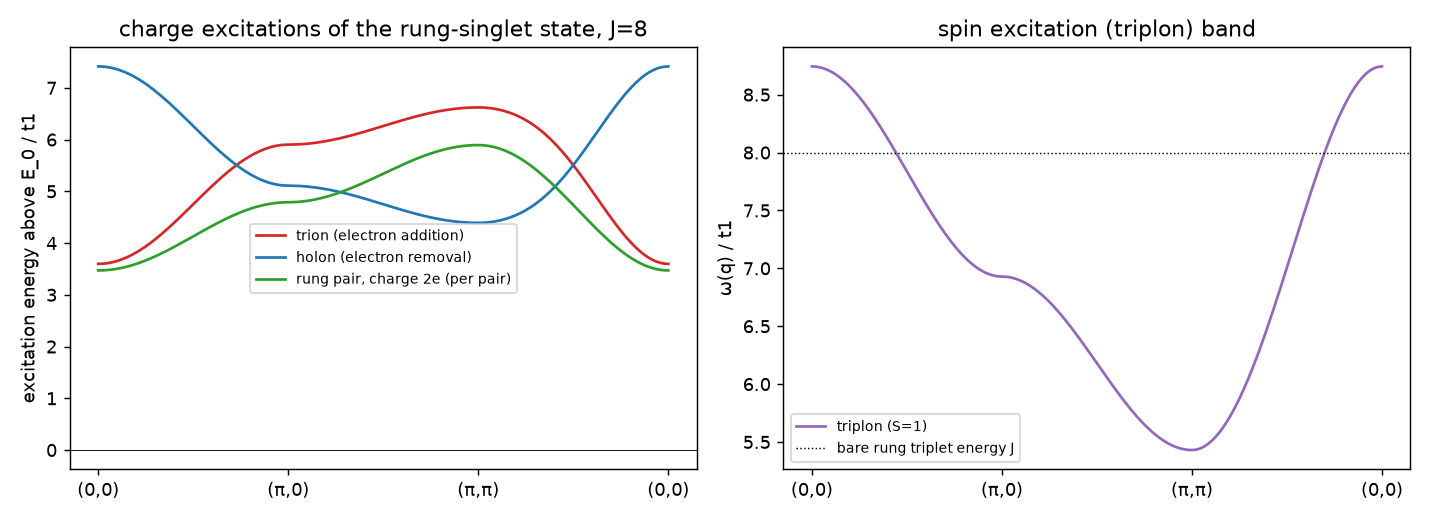
\includegraphics[width=0.95\textwidth]{figures/bands_J8.png}\end{center}

Validation on the 3$\times$2 open bilayer (24 spin-orbitals, exact Lanczos): at J=8 the exact single-particle gap is 9.74 and the spin gap 6.50, while the effective bands evaluated on the same cluster give 9.56 and 6.41; at J=6, 6.98/4.33 exact versus 6.72/4.17. The strong-coupling theory is therefore accurate to 2--4 \% for J $\ge$ 6 and degrades towards the transition (its own pair gap closes at J $\approx$ 4.9, Fig. \texttt{figures/sc\_gaps\_vs\_J.png}).
\begin{center}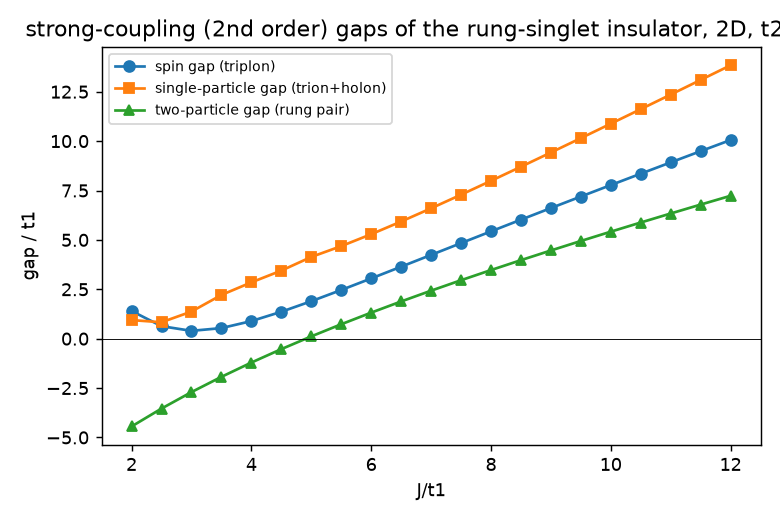
\includegraphics[width=0.95\textwidth]{figures/sc_gaps_vs_J.png}\end{center}

\subsection*{6.2 The three spectra}

The three curves are in \texttt{figures/spectra\_J8.png} (and \texttt{data/spectra\_J8.json}): STM conductance, local spin spectral function, and resistivity with its Arrhenius plot, each with the exact 3$\times$2-cluster spectrum overlaid where one exists.
\begin{center}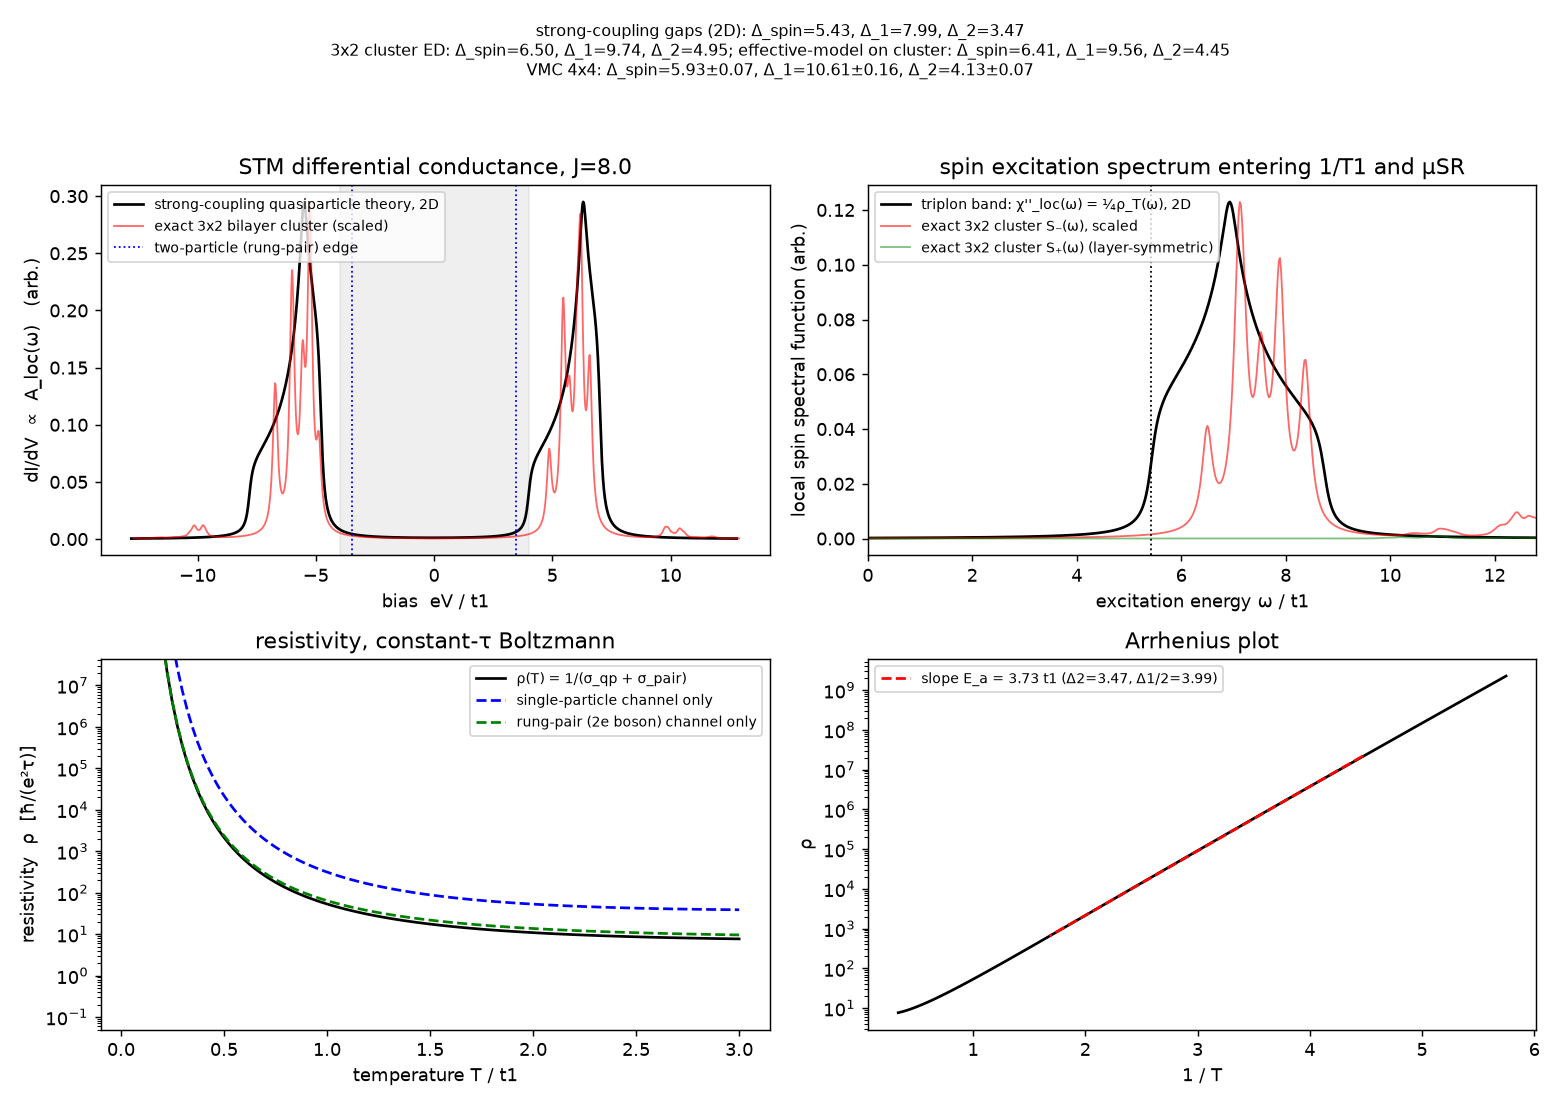
\includegraphics[width=0.95\textwidth]{figures/spectra_J8.png}\end{center}

\begin{itemize}
\item \textbf{Scanning tunnelling (dI/dV versus bias).} A\_loc($\omega$) = 1/2$\rho$\_trion($\omega$ -- $\mu$) + 1/2$\rho$\_holon($\mu$ -- $\omega$): at leading order the
trion exhausts the electron-addition weight $\langle$c c$^\dagger$$\rangle$ = 1/2 of a half-filled orbital and the holon the removal
weight, so dI/dV shows two quasiparticle bands separated by the single-particle gap $\Delta$$_1$ = min $\varepsilon$\_e + min $\varepsilon$\_h,
with van Hove peaks of the half-width t$_1$-like bands; $\mu$ is placed at mid-gap. The two-particle (rung-pair) edge
at $\pm$$\Delta$$_2$ lies \emph{inside} the single-particle gap but carries no single-electron tunnelling weight; it would appear
only in Andreev/pair tunnelling.
\item \textbf{Spin excitation spectrum (NMR 1/T$_1$, $\mu$SR).} The local dynamical susceptibility of one layer is
$\chi$''\_loc($\omega$) = 1/4 $\sum$\_q S$_-$$_-$(q,$\omega$)/N\_c = 1/4 $\rho$\_triplon($\omega$): a band of width $\approx$ 8b$_1$ + 8b$_2$ starting at the spin gap
$\Delta$\_s = $\omega$($\pi$,$\pi$), with the layer-symmetric channel empty. 1/T$_1$ follows from intraband triplon scattering,
1/T$_1$ $\propto$ $\int$d$\omega$ $\rho$\_T($\omega$)$^2$ n\_B($\omega$)[1+n\_B($\omega$)] $\propto$ e\^{}\{--$\Delta$\_s/T\} at low T.
\item \textbf{Resistivity.} Boltzmann transport with a constant relaxation time and intrinsic (mid-gap) chemical potential,
summing the charge-e quasiparticle channel (trion + holon bands, Fermi statistics) and the charge-2e rung-pair
channel (Boltzmann gas with the pair bands). $\rho$(T) is activated, $\rho$ $\propto$ exp(E\_a/T) with E\_a = min($\Delta$$_1$/2, $\Delta$$_2$); at
J=8 the fitted slope is 3.7 t$_1$, between $\Delta$$_2$ = 3.5 and $\Delta$$_1$/2 = 4.0, so the rung pairs dominate the low-T
conduction. Only the T-dependence is predicted; the prefactor $\hbar$/(e$^2$$\tau$) is not.
\end{itemize}

\section*{7. Summary, limitations, and what would settle the open points}

\subsection*{7.1 Limitations of this calculation (stated so the numbers can be weighed)}

\begin{itemize}
\item \textbf{Lattice size.} The phase assignments rest on the 4$\times$4 bilayer (32 sites); the 6$\times$6 bilayer was attempted only
at half filling and J = 4 (Sec. 3.6). Finite-size gaps on 4$\times$4 are of order 1; a gap is called
"open" only when it clearly exceeds the J = 0 value of the same cluster, and "closed" only when it falls below
it. Transition couplings are therefore intervals, not numbers.
\item \textbf{Variational bias.} The neural-Jastrow $\times$ geminal state reproduces exact 2$\times$2 energies to 0.2--0.5 \% and the
exact free-band and free-triplet energies on 4$\times$4, but it recovers only 40--55 \% of the second-order correlation
energy of the Fermi liquid, and at J $\ge$ 6 it lies $\approx$ 0.04--0.06 per site above the second-order strong-coupling
energy. Both biases are small on the scale of the energy differences between phases (0.16 per site between
the two optimized minima at J = 4) but they inflate the strong-coupling gaps by up to $\approx$ 1 and can shift the
SC--insulator boundary by a few tenths in J. A neural backflow would reduce both; it costs $\approx$ 4$\times$ per run and was
not affordable for a full phase diagram in the available time.
\item \textbf{Metastability.} Two optimizations (Fermi-liquid and rung-singlet starts) were run for every ground state;
the split between them is reported. Where it is large (J = 3--4 at half filling) the energy landscape has two
minima, which is itself a diagnostic of the first-order-like competition between the paired and unpaired
states, but it also means a third minimum cannot be excluded.
\item \textbf{Symmetric ansatz.} The pairing function, the two-body Jastrow and the RBM are all translation invariant
(with the twisted-boundary sign structure) and the state is a spin singlet-type geminal, so the variational
state cannot break translation or spin-rotation symmetry spontaneously. Magnetic or density order can show
up only as a structure-factor peak that grows with the cluster, which is what was checked (S$_-$($\pi$,$\pi$),
S$_+$($\pi$,$\pi$), N($\pi$,$\pi$) on 4$\times$4 and 6$\times$6); an explicitly symmetry-broken trial state (staggered pairing component) was
not run. With t$_2$ = 0.2 removing the nesting this is a limited risk, but it is a limitation of the test.
\item \textbf{Excited sectors.} Gaps are differences of separately optimized ground states in fixed (N$_1$,N$_2$,S\^{}z) sectors.
The spin sector uses a Pfaffian-type triplet block with both a Fermi-liquid-triplet and a triplon component and
is evaluated at total momentum (0,0) and ($\pi$,$\pi$) only; the odd sectors use one unpaired orbital.
\item \textbf{Spectra.} The three spectra are not VMC observables; they come from the strong-coupling quasiparticle theory
whose gaps are checked against exact 3$\times$2 cluster diagonalization (2--4 \% at J = 8) and against the VMC gaps.
Only the shape and the energy scales are predicted; the resistivity prefactor needs a relaxation time.
\item \textbf{Weak coupling.} "Fermi liquid" on these lattices means no resolvable pairing; the BCS gap is below the
level spacing for J $\lesssim$ 2 at $\nu$ = 1/2 and for J $\lesssim$ 3 at $\nu$ = 1/4.
\end{itemize}

\subsection*{7.2 What would settle the open points}

An 8$\times$8 bilayer at J = 4 and 5 at half filling (two-particle gap versus 1/N), a backflow-dressed ansatz at the same points, and a direct measurement of the pair superfluid stiffness (twist response) would pin the SC--insulator boundary; at quarter filling the same stiffness plus the density structure factor at ($\pi$,$\pi$) would decide superfluid versus pair crystal at large J.

\section*{8. Data, code and reproducibility}

\begin{itemize}
\item \texttt{code/model.py} (Hamiltonian term list, lattice, boundary phases), \texttt{code/ed.py} (exact diagonalization),
\texttt{code/vmc.py} (ansatz, sampler rule, observables), \texttt{code/run\_point.py} (one optimization + measurement),
\texttt{code/batch.py} (plans), \texttt{code/analyze.py} (gaps, structure factors, n(k)), \texttt{code/strong\_coupling.py} and
\texttt{code/spectra.py} (two-rung amplitudes, quasiparticle bands, cluster cross-check, spectra),
\texttt{code/pt2\_fl.py} (exact second-order perturbation theory on the cluster), \texttt{code/bcs\_weak.py} (mean-field gap).
\item \texttt{data/<L>\_<bc>\_nu<ν>\_J<J>\_<sector>.json} --- one file per optimized state with energy, error, autocorrelation,
optimization history and all measured correlators; \texttt{.mpack} holds the parameters. \texttt{data/summary.json} is the
per-point table produced by \texttt{code/analyze.py}; \texttt{data/phase\_labels.json} the labels; \texttt{data/validation\_2x2.md}
the exact-diagonalization benchmark; \texttt{data/spectra\_J8.json} the spectra curves.
\item Figures in \texttt{figures/}; this report in \texttt{report/report.md} (PDF built by \texttt{code/md2pdf.py}).
\item Environment: Python 3.11, NetKet 3.23, JAX 0.10.2, 64-core AMD EPYC node with two H200 NVL GPUs. All production
runs used the CPU backend, pinned to 4 cores per job (8 for 6$\times$6) with 15 jobs in parallel, $\approx$ 300 optimizations of
15--50 minutes each. The CPU backend was not a benchmarked choice: both GPUs were fully occupied by other users
(100\% utilization, > 100 GB each) when the project started. A timing test done afterwards on one idle H200
(\texttt{code/bench\_device.py}, production settings) gives per SR iteration: 4$\times$4 (1360 parameters, 2048 samples)
0.63 s on the GPU vs 8.9 s on 4 isolated CPU cores ($\approx$ 12 s under the production load of 15 concurrent jobs);
6$\times$6 (3040 parameters, 1024 samples) 3.2 s on the GPU vs 47 s on 8 CPU cores, i.e. a 14--15$\times$ speed-up per
optimization step. The final observable measurement (spin, n(k), pair and local correlators, 4096 samples,
4$\times$4) takes 444 s on 4 CPU cores and 2.9 s on the GPU, a 150$\times$ ratio, because the $\approx$ 100 translation-averaged
correlator operators are evaluated one after another; in production this stage was about a third of the
wall-clock time of every 4$\times$4 point. On the GPU the 6$\times$6 state needs \texttt{chunk\_size = 128}: the
translation-symmetrized RBM evaluates 36 translations $\times$ 1873 connected configurations $\times$ 1024 samples at once,
a 74 GiB intermediate that fits in host RAM but not in the default device allocation. For the 4$\times$4 sweep the
15-way CPU parallelism recovers most of the difference in throughput; for the 6$\times$6 sector runs it does not,
and any follow-up at 6$\times$6 or 8$\times$8 should run on the GPU.
\end{itemize}
\end{document}
